\section{Preliminaries}
Let $\vecs\xi \in \mathbb{R}^N$ describe the generalized state of the system with $N \geq 2$ dimensions, e.g., the robot's joint positions or the Cartesian space position.
The function $\vecs f(\vecs \xi): \mathbb{R}^N \rightarrow \mathbb{R}^N$ represents a soothly defined dynamical system (DS) describing the desired velocity at a given state $\vecs \xi$.  
%Furthermore, all trajectories converge to the unique attractor state $\vecs \xi ^a \in \mathbb{R}^N$. 

\subsection{Obstacle Avoidance}
Dynamic obstacle avoidance for point-like agents has been proposed in \cite{huber2022avoiding}. A collision-free path is obtained by modulating the base velocity $\vect f^b(\vecs \xi)$ to obtain the desired velocity:
\begin{equation}
  \vecs f(\vecs \xi) = \textbf{E}(\vecs \xi) \text{diag} \left(\lambda^r, \lambda^e, ..., \lambda^e \right) \textbf{E}(\vecs{\xi})^{-1} \vect f^b(\vecs \xi)
  \label{eq:modulated} 
\end{equation}

The orthonormal basis matrix $\textbf{E}(\vecs \xi)$, defined as:
\begin{equation}
\textbf{E}(\vecs \xi) = \left[ \textbf{r}(\vecs \xi) \ \textbf{e}_1(\vecs \xi) \ ... \ \textbf{e}_{d-1}(\vecs \xi) \right]
\label{eq:matrix_E}
\end{equation}
where the tangent directions $\textbf{e}_{(\cdot)} \in \mathbb{R}^N$ are perpendicular to the surface normal $\vect n(\vecs \xi)$, see Fig.~\ref{fig:resultant_normal}. The reference vector $\textbf{r}(\vect{\xi}) =  \left( \vecs{\xi}-\vecs{\xi}^r \right) / \| \vecs \xi-\vecs \xi ^r \|$ is pointing towards the the reference point $\vecs \xi^r \in \mathbb{R}^N$, a point placed inside the obstacle's kernel space \cite{huber2023avoidance}.

The eigenvalues in reference direction $\lambda^r$ and tangent direction $\lambda^e$ are evaluated as follows:
\begin{equation}
\begin{split}
    \lambda^r(\vecs \xi) = 1 - 1 /\Gamma(\vecs \xi) , \quad \lambda^e(\vecs \xi) = 1 + 1 / \Gamma(\vecs \xi)
    \label{eq:eigenvalues}
    \end{split}
\end{equation}
with the continuous distance function $\Gamma(\vecs \xi) \in \mathbb{R}$, which has a value of $\Gamma(\vecs \xi) = 1$ on the boundary of an obstacle, and $\Gamma(\vecs \xi) > 1$ away from the surface (Fig.~\ref{fig:resultant_normal}). In this work, we use the following distance function
\begin{equation}
  \Gamma(\vecs \xi) = 1 + \| \vecs \xi - \vecs \xi^b \|  
  \quad \text{with} \quad
  \vecs \xi^b = b (\vecs \xi - \vecs \xi^r) + \vecs \xi^r
  \label{eq:distance_function}
\end{equation}
with $b \in \mathbb{R}_{>0}$, such that $\vect \xi^b \in \mathbb{R}^N$ lies on the surface of the obstacle.

As $\lambda^r(\vecs \xi) \leq 1$, the velocity is decreased towards the obstacle, and with $\lambda^e(\vecs \xi) \geq 1$, the velocity is increased in tangent direction. It has been shown in \cite{huber2022avoiding} that this leads to convergence around (star-shaped) obstacles.

\begin{figure}
\centerline{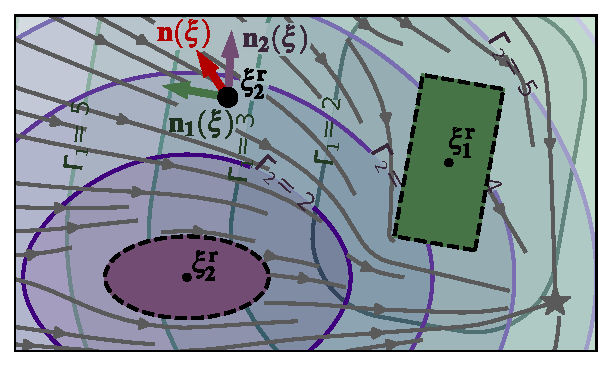
\includegraphics[width=0.5\textwidth]{figures/normal_and_gamma_field_visualization_annotated.pdf}}
\caption{
The $\Gamma$-field is defined individually for each of the obstacles. At each position $\vecs \xi$, we can evaluate the surface normals $\vect n(\vecs \xi)$. 
The desired velocity $\vect f(\vecs \xi)$ (gray) is avoiding collision with the obstacles and converges towards the attractor (black star).}
\label{fig:resultant_normal}
\end{figure}

\subsection{Force Control}

\subsubsection{Rigid Body Dynamics}
A physical system requires an interaction force that moves it around. Hence, general second-order dynamical equations are given by:
\begin{equation}
\matd{M}(\vecs\xi)\vecs{\ddot\xi} + \matd{C}(\vecs\xi, \vecs{\dot\xi})\vecs{\dot\xi} + \vect g(\vecs\xi) = \vecs{\tau_c} + \vecs{\tau_e}
 \label{eq:robot_dynamics}
\end{equation}
where we have the mass matrix of the robot $\matd M(\vecs\xi) \in \mathbb{R}^{N \times N}$, the Coriolis matrix $\matd C(\vecs\xi,\vecs{\dot\xi}) \in \mathbb{R}^N$, the gravity vector $\vect g(\vecs\xi) \in \mathbb{R}^N)$, the control torque $\vecs{\tau_c} \in \mathbb{R}^N$, and the external torque, also referred as disturbance, $\vecs{\tau_e} \in \mathbb{R}^N$.

\subsubsection{Passive Control}
Passive interaction control \cite{kronander2015passive} offers a powerful method for computing control forces from a velocity vector field. This controller provides selective disturbance rejection based on the direction of motion. Typically, the controller is configured with high damping along the direction of motion, ensuring rapid convergence of the robot's velocity to the desired value and thereby achieving excellent tracking performance. In contrast, the controller exhibits high compliance in the direction perpendicular to the motion, enabling flexible behavior and greater resistance to external forces. This versatile approach enables robots to adeptly navigate dynamic environments while maintaining stable and precise control, making it a valuable asset for a wide range of robotic applications.
% Passive interaction control \cite{kronander2015passive} enables computing a control force from a velocity vector field. The controller allows selective disturbances rejection, given the direction of motion. Most commonly, the controller is set to have high damping in the direction of the motion but be compliant in the direction perpendicular to the motion. High damping implies results in the robot's velocity rapidly converging to the desired velocity, leading to good tracking performance. Conversely, high compliance results in flexible behavior and resist little to external forces.

The passive control force \cite{kronander2015passive} is given as:
\begin{equation}
	\vecs{\tau_c} = \vect g (\vecs\xi) 
	% + \matd{D}(\vect \xi, \dot{\vect \xi}) \dot{\vect \xi}  
	+ \matd{D}(\vecs\xi) \left(\vecs f(\vecs\xi) - \vecs{\dot\xi} \right) 
\label{eq:control_command}
\end{equation}
This control law embeds a gravity compensation term and a damping term, which decreases the difference between the desired velocity $\vecs f(\vecs\xi)$ and the actual velocity $\vecs{\dot\xi}$.

The positive definitie damping matrix $\matd D(\vecs\xi) \in \mathbb{R}^{N \times N}$ is designed to allow for damping in each sub-direction:
\begin{equation}
   \matd {D}(\vecs \xi) = \matd{Q}(\vecs\xi)\matd{S}(\vecs\xi) \matd{Q} (\vecs \xi)^{-1}
\label{eq:damping_matrix}
\end{equation}
where $\matd Q(\vecs \xi) \in \mathbb{R}^{N \times N}$ is an othonormal basis matrix. 
formed by $\vecs{q}_1, \vecs q_2, ..., \vecs q_N$ The first vector is pointing in the desired direction of motion: $\vecs q_1 = \dot{\vecs \xi} / \lVert \dot{\vecs \xi} \rVert$.

The diagonal matrix $\matd{S}(\vecs\xi) \in \mathbb{R}^{N \times N}$ consists of damping factors in the corresponding direction.
Increase consistency with the desired velocity s achieved, by setting the first damping factor $s_1 \geq 0$ to a high value. The damping in the remaining directions $s_i \geq 0$ with $i = 2 .. N$ is set lower to allow compliance perpendicular to the motion. 

\subsection{Stability Analysis} \label{sec:trad_passive}
It is crucial to consider varying control parameters carefully, as they can inject energy into a system, potentially leading to unstable behavior \cite{ferraguti2013tank}. Ensuring stability guarantees is of paramount importance to safeguard both the hardware and the environment in which the control system operates.

In human-robot interaction, the robot faces external disturbances of unknown nature. To achieve stable and bounded behavior in the face of such disturbances, \textit{passivity} analysis proves to be a valuable tool. By employing passivity analysis, the control system can be designed to maintain stable responses (bounded system) in the presence of any external force (bounded input). This property enhances the reliability and safety of the control system, making it more resilient in dynamic and uncertain environments.

\begin{definition}[Passivity \cite{willems1972dissipative, sepulchre2012constructive}]
  A dynamical system with input $ u \in \mathcal{U}$ and output $y \in \mathcal{Y}$ is passive with respect to the supply rate $s : \mathcal{U} \times \mathcal{Y} \rightarrow{R}$ if, for any $u: \mathbb{R}_{>0} \rightarrow \mathcal{U}$ and any time $t \geq 0$ the following is satisfied
  \begin{equation}
    \int_0^t s \left( u(\tau),  y (\tau) \right) d \tau \leq c^2
  \end{equation}
  where $c \in \mathbb{R}$ depends on the initial conditions.
\end{definition}

Since two passive systems result in a passive system \cite{sepulchre2012constructive}, by ensuring that a controller is passive it follows that its interaction with its (passive) environment results in a passive system.
